\documentclass[conference]{IEEEtran}
\IEEEoverridecommandlockouts
% The preceding line is only needed to identify funding in the first footnote. If that is unneeded, please comment it out.
\usepackage{cite}
\usepackage{amsmath,amssymb,amsfonts}
\usepackage{algorithmic}
\usepackage{graphicx}
\usepackage{textcomp}
\usepackage{xcolor}
\usepackage{booktabs}
\def\BibTeX{{\rm B\kern-.05em{\sc i\kern-.025em b}\kern-.08em
    T\kern-.1667em\lower.7ex\hbox{E}\kern-.125emX}}
\begin{document}

\title{Mobile-PIRL: Mobile Versions of Pretext-Invariant
Representation Learning - Progress Report\\
}

\author{\IEEEauthorblockN{İzzet Emre Küçükkaya}
\IEEEauthorblockA{
\textit{Boğaziçi University}\\
Istanbul, Turkey \\
izzet.kucukkaya@boun.edu.tr}
\and
\IEEEauthorblockN{Berkcan Üstün}
\IEEEauthorblockA{
\textit{Boğaziçi University}\\
Istanbul, Turkey \\
berkcan.ustun@boun.edu.tr}
}

\maketitle


\section{Related Work}
\textbf{Self-Supervised Learning}. The supervised learning techniques requires large amount of semantically annotated data such as class labels, bounding boxes or hashtags which is a compelling need in order to perform efficiently. The Self-Supervised learning techniques are introduced to overcome this obstacle. The goal of the Self Supervised Learning is to learn comprehensive representations of the samples without the need of semantically annotated data. Sparse coding \cite{50}, adversarial training \cite{11}, auto-encoders \cite{Masci11stackedconvolutional}, and probabilistic variations of these methods \cite{59} have all been used to recreate pictures from a tiny, intermediate representation. 

\textbf{Pretext Learning}. In recent years, the methods that constructs the representations without annotation have shifted to learning with the pretext tasks \cite{9}. Many pretext tasks can be enumerated, namely, ordering video frames \cite{pirl1} for video data or predicting contextual image patches \cite{pirl9} for image data. A simpler pretext task involves applying an image transformation (data augmentation) to the input sample and predicting it \cite{pirl76}. 

\textbf{Contrastive Loss}. The base method PIRL uses a contrastive loss \cite{pirl22}. Many of the methods that uses the contrastive loss involves predicting the  lost parts of the input samples such as predicting future frames in a video \cite{pirl23} or operate on multiple views \cite{pirl64}. 

\textbf{Mobile Networks}. Visual classification and pattern recognition applications are essential in some studies that require mobility such as augmented reality. In this context, it is essential that convolutional neural networks, which are the cornerstone of visual classification and pattern recognition applications, become capable of responding to this mobility need. Within the scope of this need, structures that are variable and effective in terms of the number of arithmetic operations performed, have a light computational load and can work quickly have been developed. \cite{mobile3,efficientnet,mnasnet,shuffle}, can be considered as the examples of these works.  


\begin{figure}[h]
\centerline{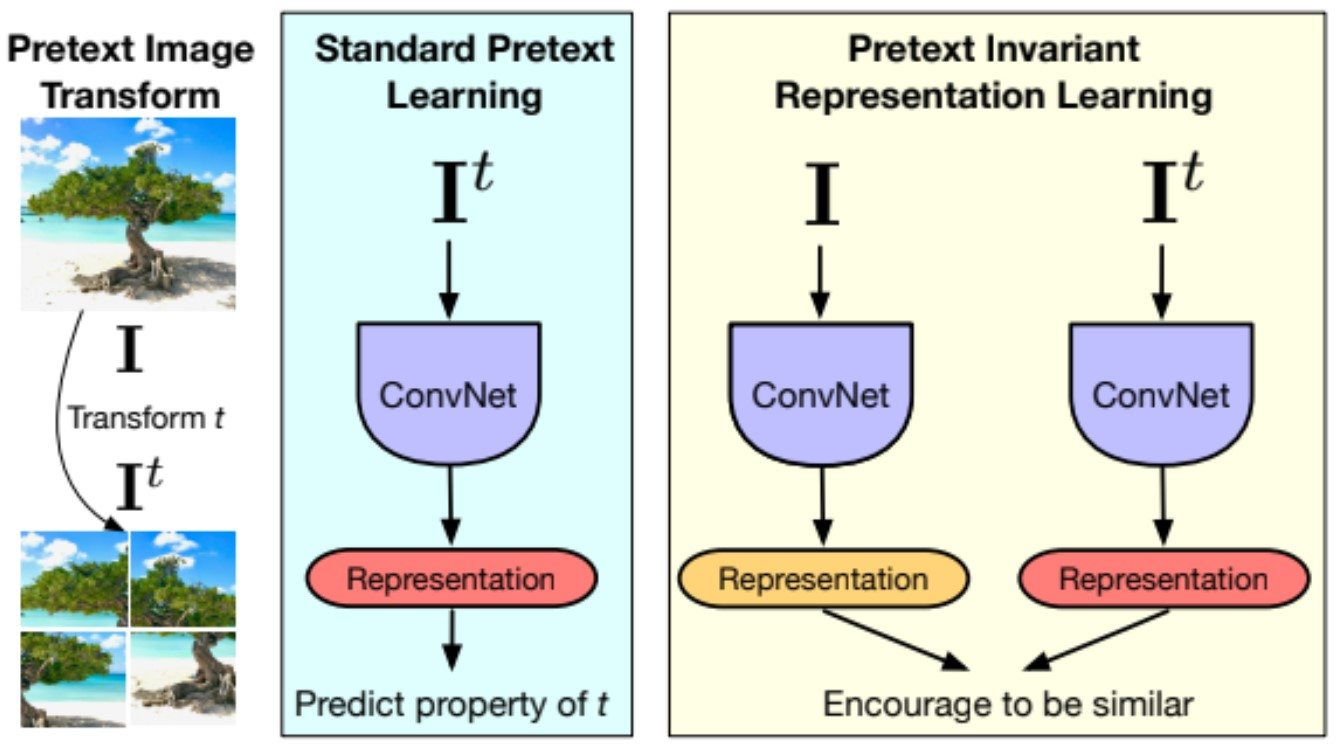
\includegraphics[width=8cm]{fig1.jpg}}
\caption{Comparison of the Standard Pretext Learning and Pretext Invariant Representation Learning \cite{PIRL}}
\label{fig}
\end{figure}

\begin{figure}[h]
\centerline{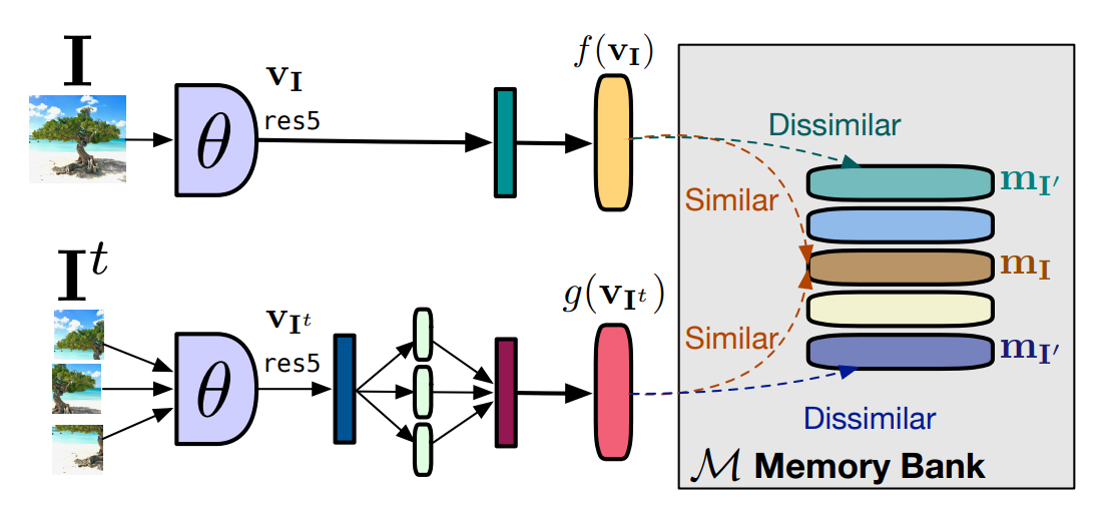
\includegraphics[width=8cm]{PIRL_arch.png}}
\caption{Architecture of PIRL \cite{PIRL}}
\label{fig_PIRL_arch}
\end{figure}

\begin{figure*}[h]
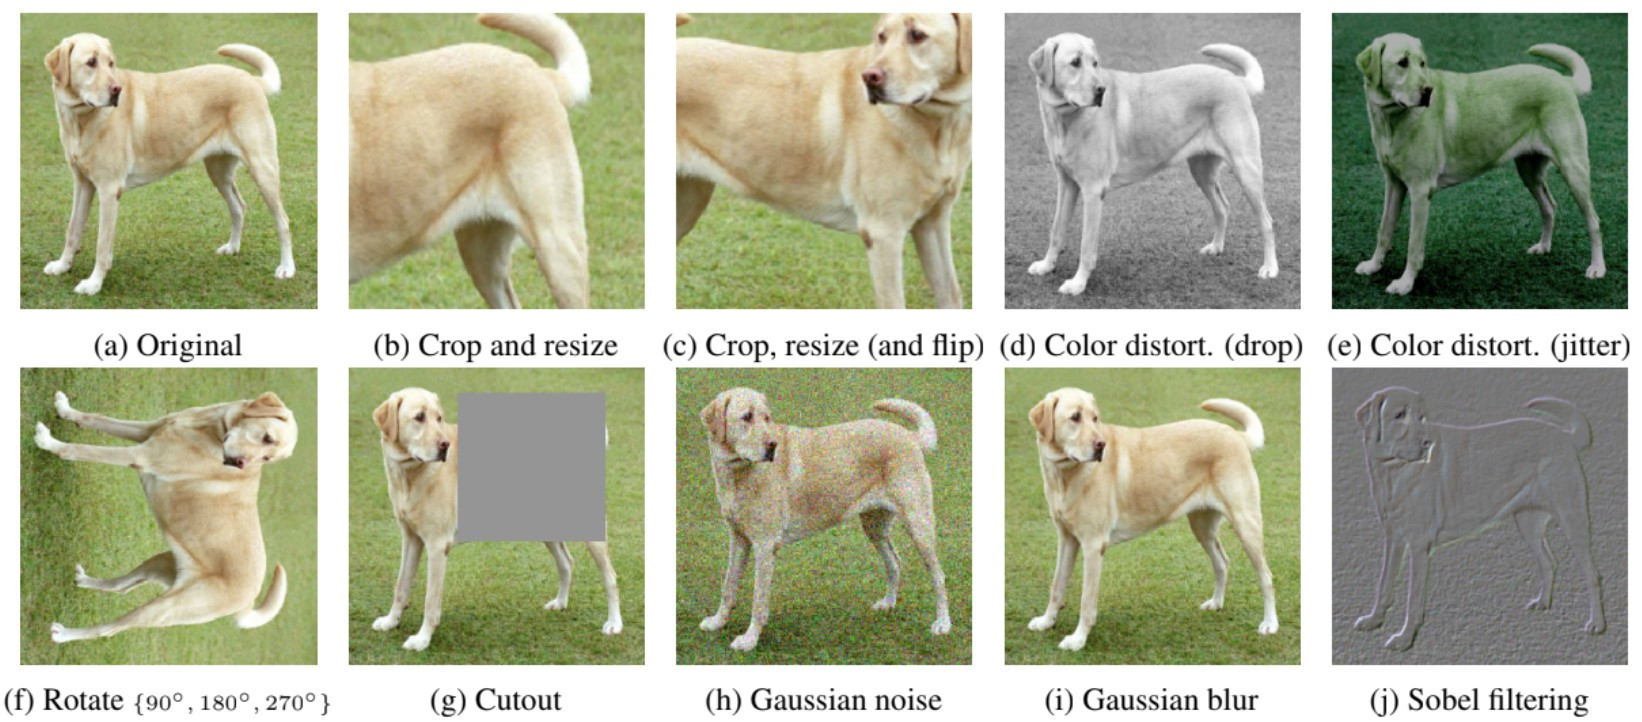
\includegraphics[width=\textwidth]{fig2.jpg}
\centering
\caption{Examples of data augmentations \cite{SimCLR}}
\label{fig2}
\end{figure*}




\section{Method}
\subsection{Pretext Tasks in Detail}
In the most of the self supervised techniques the pretext tasks are used. In computer vision, pretext tasks are tasks that are designed so that a network trained to solve them will learn visual features that can be easily adapted to other downstream tasks. A Downstream is a task that typically has real world applications and human annotated data.There are many different kinds of pretext tasks. The simplest ones typically involve augmentation of the input data and then training a network to learn what augmentation has been applied, examples can be seen from the Figure \ref{fig2} and include rotation, color removal, Gaussian noise, Gaussian blur and more. This way we can generate both the input and the solution to the chosen task, automatically. In the pearl, authors used jigsaw transformation.

\subsection{Pretext Invariant Representation Learning}
\textbf{Overview}. It is mentioned that the simplest pretext task is the predict what augmentation has been done and this is the main idea of basic pretext learning. On the other hand, PIRL proposes a new idea that learning representations which is invariant to the transformation is a better idea than predicting the what transformation has been applied. The overview of this can be seen in the Figure \ref{fig}. This way, PIRL tries to construct representations that do not vary with the applied affine transformation to the input data. If the input data has an object, the output representation will be the same as if the object rotates, scales or shifted in color space. This becomes crucial in the sense of constructing a comprehensive representation of the objects. 

\textbf{Loss Function}. The loss function of the PIRL is implemented by using a contrastive loss function $L(.,.)$ \cite{pirl22}. It can be demonstrated as;

\begin{equation}\label{eq: loss_nce}
\begin{aligned}
    L_{NCE}(I,I^t) = - \log[h(f(v_I),g(v_I^t)] - 
\\
    \sum_{I' \in D_N} \log[1- h(g(v_I^t),f(v_{I'}))]
    \end{aligned}
    \end{equation}
This loss function coerces the representation of the image $I$ to be similar to the representation of its transformed version $I^t$, while discourages it to be similar to the representations of the other images in the dataset $I'$.  Here, the NCE stands for the Noise Constractive Estimator. Spesifically, the method defines a matching score that measures the similarity between two representations and uses this score in the noise constractive estimator which models the binary event that $(I,I^t)$ originates from some distribution. In the (NCE), each “positive” sample $(I, I^t )$ has N corresponding “negative” samples. The negative samples are obtained by computing features from other $I' \neq I$.

\subsection{Memory Bank}\label{membank}
PIRL uses Resnet-50 as the backbone architecture which will be replaced by us with mobile networks. Both of the original image and the transformed image goes into the Resnet and the bunch of layers afterwards as we can be seen in the Figure \ref{fig_PIRL_arch}. Then we expect that $f(v_I)$ and $g(v_{I^t})$ are similar. Therefore a memory bank is defined which is the moving average of $f(v_I)$ among epochs. The similarity is checked comparing the representations with that moving average values.

\subsection{Overall Implementation}
The PIRL uses the Jigsaw transformation as the primary data augmentation. The authors also include the rotation transformation in order to demonstrate the generalization of the proposed method. The image representation $I$ is obtained by the linear projection of the ResNet features to the 128-dimensional vector. In order to calculate the representation of the transformed image $I^t$, nine patches are extracted from the image and goes to the ResNet one by one. The 128-d vectors are obtained for each patch. Those vectors are concatenated in a random order followed by second projection to again 128-d vector.  


\section{Experiments}
The experiments have been done in google colab environment (pro) which uses Tesla P100 GPU cores with 16GB memory. The STL-10 dataset is chosen which consists of 100.000 unlableled images for self-supervised learning and 5.000 images which are labeled with 10 classes for fine-tuning \cite{stl10}. The method with memory bank in \ref{membank} is implemented to conduct experiments. The backbone architectures are replaced with the architectures with less number of parameters. 2 different models for each architecture is trained. Primary is the PIRL model which is trained self-supervised. The training of the PIRL model takes lots of time due to the dataset and its complexity compared to the secondary model. Secondary model is the fine-tuned version of the primary model using labeled dataset. The backbone architecture of the secondary model is extracted from the primary model to generate 128 dimensional representations and added a linear layer to do classifications to 10 classes using that representations.\\
\begin{figure}[h]
\centerline{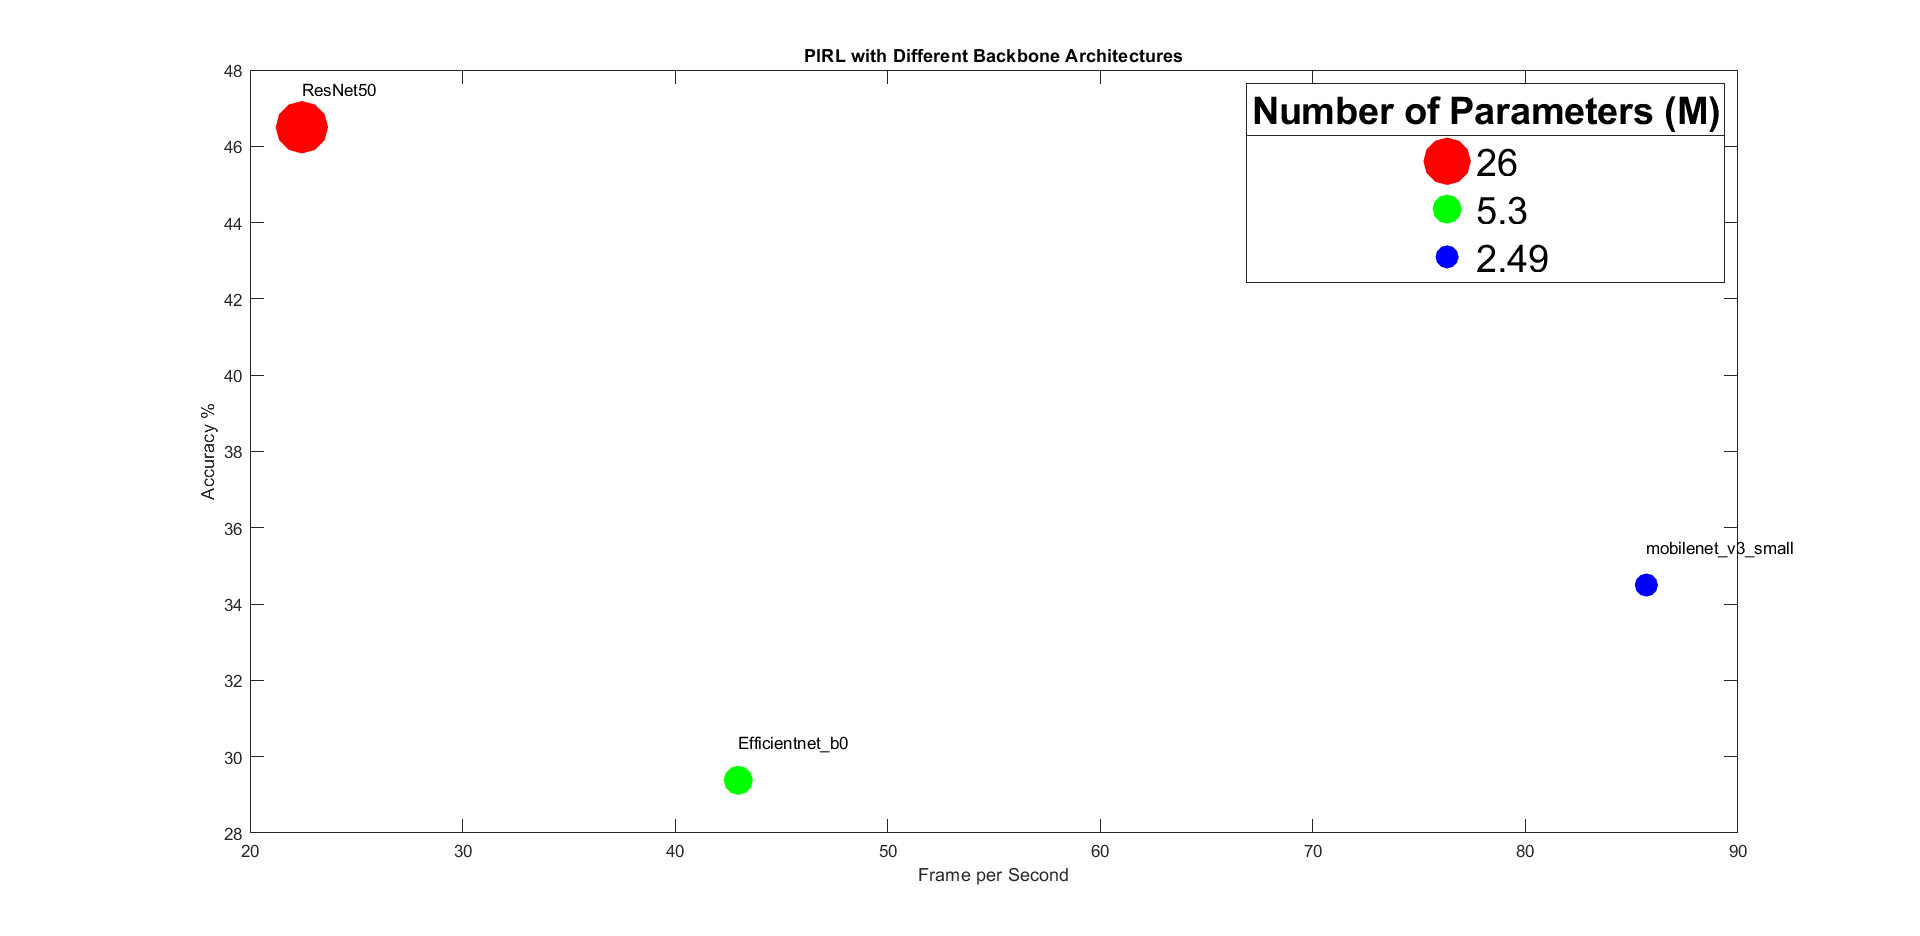
\includegraphics[width=8cm]{results.png}}
\caption{Comparison of PIRL Backbone Architectures}
\label{fig_results}
\end{figure}
Results of the experiments can be seen in the Fig. \ref{fig_results}. The size of the circles represents the number of parameters, x axis represents the number of batches can be processed within a second and y axis represents the test set accuracy. As can be seen, although the number of parameters is decreased to its 1/10, the accuracy of the experiment with mobilenet\_v3\_small is not decreased that much. Furthermore, the number of frames tested within a second using mobilenet\_v3\_small is 4 times greater than the number of frames tested within a second with ResNet50 architecture.
\section{Next Steps}
The experiments are done using several mobile network architectures. However, there are several more promising architectures as mentioned in section 1. We are planning to test these architectures first and continuing to train models and do experiments. Furthermore, as mentioned before, we are planning to do other pretext tasks and combination of those and check if they improve the results and make representations more pretext-invariant.
\bibliographystyle{IEEEtran}
\bibliography{sample}
\vspace{12pt}

\end{document}